% !TeX root = vpl.tex

\chap{Multiple Sensor Thresholds}\label{ch.slow}

As explained in \cref{a.tech}, in advanced mode sensors events can be
specified in three different ways: an event occurs when the reflected
light is below a threshold (black), an event occurs when the reflected
light is above a threshold (white), and an event occurs when the
reflected light falls between two thresholds (dark gray):

\begin{center}
\begin{tabular}{ccc}
\blk{slow-low}&\blk{slow-mid}&\blk{slow-high}\\
\end{tabular}
\end{center}

\bigskip

\textbf{Specification}

Construct a program that causes the robot to approach an object,
starting at a high speed, slowing down as it gets closer, and finally
stopping when the robot is very close to the object.

\textbf{Guidance}

\begin{itemize}
\item Use three event-actions pairs, one with each type of sensor
event.

\item Carefully adjust the sliders (see \cref{a.tech}) so that the
high value of one threshold is the same as the low value of the next
threshold. 

\item Add a color block to each pair so that you can see the robot's
speed setting.

\item Use reflector tape to extend the range of
the sensors as explained in \cref{a.blocks}. 
\end{itemize}

\bigskip

{\raggedleft \hfill Program file \bu{slow.aesl}}

\bigskip
\bigskip

\textbf{Specification}

The line following program in Chapter~\ref{ch.line} used two sensors to decide if the robot is moving off the line to the left or to the right. Implement a line following algorithm that uses one sensor.

\textbf{Guidance}

The robot will follow the \emph{edge} of the line, not its center. The ground sensors receive reflected light from a relatively wide area so the decision can be made using multiple thresholds. If the right sensor is used to follow the right edge of a (dark) line:
\begin{itemize}
\item If the sensor is to the left of the edge, little light will sensed.
\item If the sensor is to the right of the edge, a lot of light will be sensed.
\item If the sensor is over the edge, the amount of light sensed will be midway between the two extreme values.
\end{itemize}
The three cases are shown in the following diagram:
\begin{center}
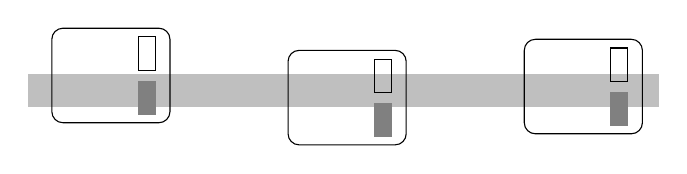
\begin{tikzpicture}
\draw[fill,lightgray] (0,0) rectangle +(8,4mm);
\foreach \x/\y in {6.5cm/1pt, .5cm/5pt, 3.5cm/-3pt} {
  \draw[rounded corners] (\x-2mm,\y-11pt) rectangle +(15mm,12mm);
  \draw[fill,gray] (\x+.9cm,\y-8pt) rectangle +(6pt,12pt);
  \draw (\x+.9cm,\y+8pt) rectangle +(6pt,12pt);
}
\end{tikzpicture}
\end{center}

\bigskip

{\raggedleft \hfill Program file \bu{line-one.aesl}}
